\documentclass{article}

% Language setting
% Replace `english' with e.g. `spanish' to change the document language
\usepackage[english]{babel}
\usepackage{float}
\usepackage{minted}
\usepackage{natbib}
\usepackage{longtable}
\usepackage{tabularray}
\usepackage{ragged2e}
\usepackage{xcolor} %% http://www.ctan.org/pkg/xcolor
% Set page size and margins
% Replace `letterpaper' with `a4paper' for UK/EU standard size
\usepackage[letterpaper,top=2cm,bottom=2cm,left=3cm,right=3cm,marginparwidth=1.75cm]{geometry}
\justifying
% Useful packages
\usepackage{amsmath}
\usepackage{graphicx}
\definecolor{darkblue}{rgb}{0.0, 0.0, 1.0}


\begin{document}


\begin{titlepage}

        \centering
    \vspace*{1cm}

    
\includegraphics[width=0.7\textwidth]{dei_thumb.png} % Replace with your university logo

    \vspace{1.5cm}
    {\LARGE \textbf{Practical Assignment \#2
} \par}
    \vspace{0.5cm}
    {\Large 2023/2024\par}

    \vspace{2.5cm}
    \textbf{Master in Informatics Engineering} \\
    \textbf{Information Technology Security} \par
    \vspace{2cm}
    \vspace{6cm}
    \begin{tabular}{ll}
        \textbf{Bruno Sequeira} & 2020235721, brunosequeira@student.dei.uc.pt \\
        \textbf{Rui Santos} & 2020225542, rpsantos@student.dei.uc.pt
        \\
    \end{tabular}

        
    \vfill
    {\large \today \par}
    \clearpage
    \tableofcontents
    \clearpage
    
\end{titlepage}



\section{Introduction}
\quad In the evolving field of Informatics Engineering, the significance of Information Technology Security cannot be overstated. This practical assignment delves into the intricate architecture and software configurations necessary to safeguard a network infrastructure. By implementing IPTables and Suricata, we aim to establish a secure environment capable of dealing with potential threats and ensuring the integrity of our system.

\section{Architecture}

\begin{figure}[H]
    \centering
    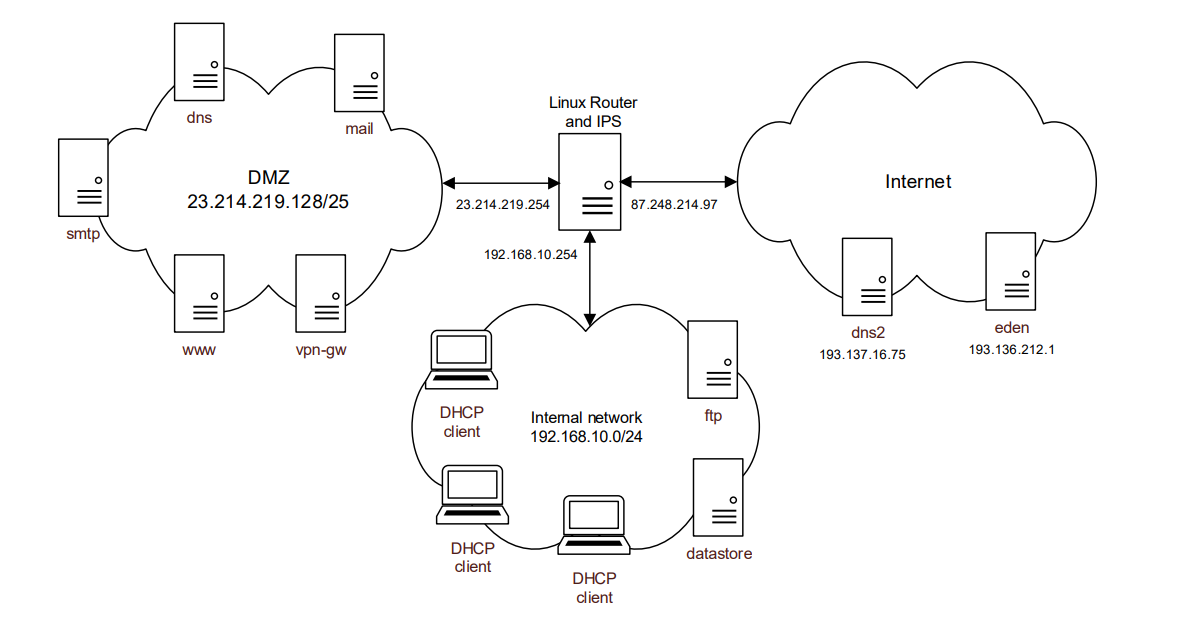
\includegraphics[scale=0.5]{pics/architecture_sti2.png}
    \caption{Network Architecture}
    \label{fig:network-arc}
\end{figure}

\quad To do this assignment, he needed three computers, one for the LinuxRouter and IDS, one for the DMZ and another for the internal network. The DMZ have the DNS, mail, smtp, www and vpn-gw servers and the Internal Network computer have DHCP clients, FTP server and a datastore. In each computer we will have a dedicated IP address for each of those services.\par
\textbf{}
\par 
Networks:
\begin{itemize}
    \item DMZ: 23.214.219.218/25
    \item External: 87.248.214.0/24
    \item Internal: 192.168.10.0/24\par
\end{itemize}
\par
Services IP:

\begin{itemize}
\item Linux Router
\begin{itemize}
\item DMZ interface: 23.214.219.254
\item internal network interface: 192.168.10.254
\item external network interface: 87.248.214.97
\end{itemize}
\item DMZ
\begin{itemize}
\item DNS: 23.214.219.130
\item mail: 23.214.219.131
\item smtp: 23.214.219.132
\item www: 23.214.219.133
\item vpn-gw: 23.214.219.134
\item external network: 87.248.214.89
\end{itemize}
\item Internal Network
\begin{itemize}
\item DHCP Client 1: 192.168.10.2
\item DHCP Client 2: 192.168.10.3
\item DHCP Client 3: 192.168.10.4
\item FTP: 192.168.10.5
\item datastore: 192.168.10.6
\item external network: 87.248.214.90
\end{itemize}

\end{itemize}


\section{Software}
\quad To complete the assignment we used three virtual machines, all CentOS Stream 9. In the LinuxRouter virtual machine we needed:

\begin{itemize}
    \item suricata: the technology that we use to detect and block attacks
    \item iptables: our firewall\par
\end{itemize}
On the other machines we needed:  
\begin{itemize}
    \item netcat: to test most of the connections
    \item vsftp: to create ftp clients and servers
\end{itemize}

\section{Concepts}
\subsection{IPTables}
\quad IPTables is a firewall that works by matching each packet that crosses the networking interface against a set of rules to decide what to do.\par
The rules define the characteristics that a packet need to have to be a match and the action to be taken.
Those rules are saved in tables. There are three tables in IPTables, \textit{nat, filter and mangle}. In this project we will only work with the first two.\par
The rules inside the tables are grouped in \textbf{chains} and users can create chains as needed, but in our case it was not necessary. In the table \textit{filter} three default chains: \textbf{INPUT,OUTPUT, FORWARD}. The chain \textbf{INPUT} handles the packets addressed to the router, the chain \textbf{OUTPUT} handles the traffic created by our router and the chain \textbf{FORWARD} handles the traffic that needs to be redirected by the router to another system. In the table \textit{nat} we have the chains \textbf{POSTROUTING} and \textbf{PREROUTING}. The \textbf{PREROUTING} chain is for altering packets before they are routed. It is used for \textbf{DNAT} for incoming traffic. The \textbf{POSTROUTING} chain is for altering packets as they are leaving the system. It is used for SNAT or outgooing traffic.\par
The rules have actions that define if a packet is dropped/rejected (\textbf{DROP}) or if a packet can proceed to his destination (\textbf{ACCEPT}).


\subsection{Suricata}
\label{subsec:suricata}
\quad Suricata is a open source network analysis and threat detection software used by multiple organizations. By default, suricata runs as an Intrusion Detection System (IDS), that means that it only generates alerts and logs of suspicious activity. We are going to configure it to also be in Intrusion Prevention System(IPS) so it can also drop the suspicious traffic. We are also going to use Suricata in inline mode, that is a mode where the packets are sent from IPTables to Suricata using a Queue and if a packet in the queue have some characteristic that matches one of the suricata's rules it will be dropped. The rules follow a format wich is as follows:\par
\begin{center}
\textbf{action protocol source(ports) $\rightarrow$ destination(ports) options}
\end{center} \par
The actions are what determines what happens when a signature matches, the protocol is what protocol does the rule apply, the source and destination are the specification of the source and destination of the traffic and the ports are the ports that the traffic comes in and out.
    


\section{IPTables Configuration}
\quad In this section we are going to show how we configured out firewall in order to meet the assignment requirements.

\subsection{Firewall configuration to protect the router}
\quad Here we want the firewall to be configured so that it should drop all communications entering the router system except the ones we are going to describe next. But first we need to change the \textbf{INPUT} chain policy to \textbf{DROP}, which means that the default action for every packet that does not match a rule in this chain is \textbf{DROP}. \par
\texttt{iptables -P INPUT DROP}

\subsubsection{DNS name resolution requests sent to outside servers}
\quad Since DNS uses both TCP and UDP protocols we made rules for both of those protocols in order to accept the incoming and outgoing DNS packets.\par
\texttt{}\par
\texttt{iptables -A INPUT -p tcp --dport 53 -j ACCEPT}\par
\texttt{iptables -A INPUT -p udp --dport 53 -j ACCEPT}\par
\texttt{}\par
In order to test the rules we used netcat and in this case we put the following commands:\par
\texttt{}\par
Router UDP: \texttt{nc -l -v -u -p 53} \par
DMZ (dns server) UDP: \texttt{nc -v -u 23.214.219.254 53} \par
\texttt{}\par
\texttt{}\par
Router TCP: \texttt{nc -l -v -p 53} \par
DMZ (dns server) TCP: \texttt{nc -v 23.214.219.254 53} \par
\texttt{}\par
And the results were:
\begin{figure}[H]
    \centering
    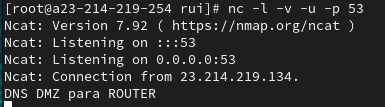
\includegraphics[scale=0.5]{in/in_dns_router.png}
    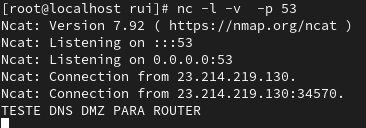
\includegraphics[scale=0.5]{in/in_dns_router_tcp.png}
    \caption{Netcat command in the Router UDP and TCP}
    \label{fig:network-arc}
\end{figure}

\begin{figure}[H]
    \centering
    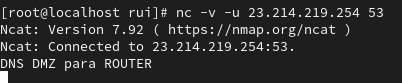
\includegraphics[scale=0.5]{in/in_dns_dmz.png}
    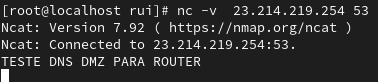
\includegraphics[scale=0.5]{in/in_dns_dmz_tcp.png}
    \caption{Netcat command in the DMZ's dns server UDP and TCP}
    \label{fig:network-arc}
\end{figure}

\subsubsection{SSH connections to the router system, if originated at the internal network or at the VPN gateway (vpn-gw).} 
\quad Here, we want to accept connections from the internal network (192.168.10.0/24) and from the VPN server (23.214.219.134) that use the SSH port.\par
\texttt{}\par
\texttt{iptables -A INPUT -s 23.214.219.134 -p tcp --dport ssh -j ACCEPT}\par
\texttt{iptables -A INPUT -s 192.168.10.0/24 -p tcp --dport ssh -j ACCEPT}
\texttt{}\par

In order to test these we used the ssh command:
\begin{figure}[H]
    \centering
    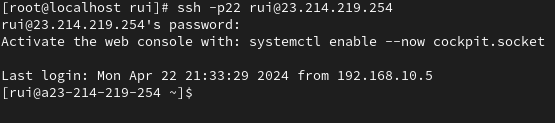
\includegraphics[scale=0.5]{in/in_ssh_dmz.png}
    \caption{SSH from vpn-gw}
    \label{fig:network-arc}
\end{figure}

\begin{figure}[H]
    \centering
    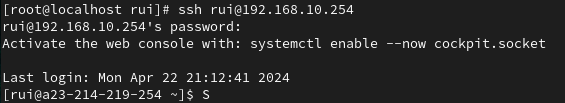
\includegraphics[scale=0.5]{in/in_ssh_internal.png}
    \caption{SSH from internal network}
    \label{fig:network-arc}
\end{figure}



\subsection{Firewall configuration to authorize direct communications (without NAT)}

\quad Here, we want our firewall to drop all communications between networks, which we did with the command:\par
\texttt{}\par
\texttt{iptables -P FORWARD DROP}\par
\texttt{}\par

However, like we did in the subsection before, there are some exceptions that we are going to describe next.

\subsubsection{Domain name resolutions using the dns server}

\texttt{}\par
\texttt{iptables -A FORWARD -d 23.214.219.130 -p udp --dport domain -j ACCEPT}\par
\texttt{iptables -A FORWARD -d 23.214.219.130 -p tcp --dport domain -j ACCEPT}\par
\texttt{iptables -A FORWARD -s 23.214.219.130 -p udp --sport domain -j ACCEPT}\par
\texttt{iptables -A FORWARD -s 23.214.219.130 -p tcp --sport domain -j ACCEPT}\par
\texttt{}\par

In order to test these we used the netcat command:
\texttt{}\par
\texttt{}\par
DMZ (dns server) UDP: \texttt{nc -l -v -u -p 53} \par
Internal Network UDP: \texttt{nc -v -u 23.214.219.130 53} \par
\texttt{}\par
\texttt{}\par
DMZ (dns server) TCP: \texttt{nc -l -v -p 53} \par
Internal Network TCP: \texttt{nc -v 23.214.219.130 53} \par
\texttt{}\par
\begin{figure}[H]
    \centering
    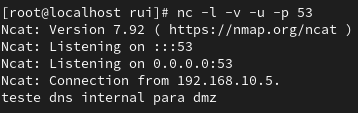
\includegraphics[scale=0.5]{btw/btw_dns_dmz.png}
    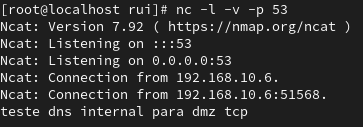
\includegraphics[scale=0.5]{btw/btw_dns_dmz_tcp.png}
    \caption{Netcat command DMZ's dns server}
    \label{fig:network-arc}
\end{figure}

\begin{figure}[H]
    \centering
    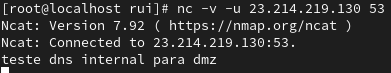
\includegraphics[scale=0.5]{btw/btw_dns_internal.png}
    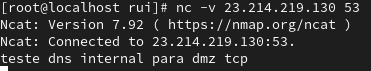
\includegraphics[scale=0.5]{btw/btw_dns_internal_tcp.png}
    \caption{Netcat command internal network}
    \label{fig:network-arc}
\end{figure}


\subsubsection{ The dns server should be able to resolve names using DNS servers on the Internet (dns2 and also others)}
\quad Here we are allowing the dns server to access the Internet to resolve names.

\texttt{}\par
\texttt{iptables -A FORWARD -s 23.214.219.130 -d 87.248.214.0/24 -p udp --dport domain -j ACCEPT}\par
\texttt{iptables -A FORWARD -s 87.248.214.0/24 -d 23.214.219.130 -p udp --sport domain -j ACCEPT}\par
\texttt{}\par

In order to test these we used the netcat command:
\texttt{}\par
\texttt{}\par
DMZ (dns server): \texttt{nc -v -u 87.248.214.89 53} \par
External Network: \texttt{nc -l -v -u -p 53} \par
\texttt{}\par
\begin{figure}[H]
    \centering
    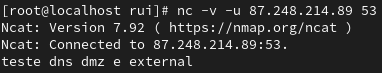
\includegraphics[scale=0.5]{btw/btw_dns_external_dmz_newip.png}
    \caption{Netcat command DMZ's dns server}
    \label{fig:network-arc}
\end{figure}

\begin{figure}[H]
    \centering
    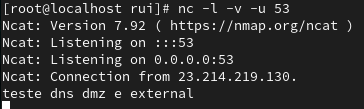
\includegraphics[scale=0.5]{btw/btw_dns_external_external_newip.png}
    \caption{Netcat command external network}
    \label{fig:network-arc}
\end{figure}



\subsubsection{ The dns and dns2 servers should be able to synchronize the contents of DNS zones.}
\quad In order to synchronize the contents of DNS zones we can use TCP ports, so the rules will be the same as before but with the port TCP instead of UDP.

\texttt{}\par
\texttt{iptables -A FORWARD -s 23.214.219.130 -d 87.248.214.0/24 -p tcp --dport domain -j ACCEPT}\par
\texttt{iptables -A FORWARD -s 87.248.214.0/24 -d 23.214.219.130 -p tcp --sport domain -j ACCEPT}\par
\texttt{}\par

In order to test these we used the netcat command:
\texttt{}\par
\texttt{}\par
DMZ (dns server): \texttt{nc -v 87.248.214.89 53} \par
External Network: \texttt{nc -l -v -p 53} \par
\texttt{}\par
\begin{figure}[H]
    \centering
    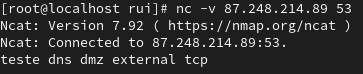
\includegraphics[scale=0.5]{btw/btw_dns_external_tcp_dmz.png}
    \caption{Netcat command DMZ's dns server}
    \label{fig:network-arc}
\end{figure}

\begin{figure}[H]
    \centering
    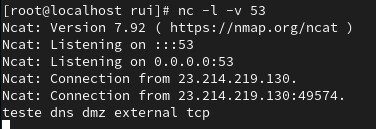
\includegraphics[scale=0.5]{btw/btw_dns_external_tcp_external.png}
    \caption{Netcat command external network}
    \label{fig:network-arc}
\end{figure}


\subsubsection{SMTP connections to the smtp server}

\quad To allow SMTP (Simple Mail Transfer Protocol) to send and receive messages we created the following rules:

\texttt{}\par
\texttt{iptables -A FORWARD -d 23.214.219.132 -p tcp --dport smtp -j ACCEPT}\par
\texttt{iptables -A FORWARD -s 23.214.219.132 -p tcp --sport smtp -j ACCEPT}\par
\texttt{}\par


In order to test these we used the netcat command:
\texttt{}\par
\texttt{}\par
DMZ (smtp server): \texttt{nc -l -v -p 25} \par
Internal Network: \texttt{nc -v 23.214.219.132 25} \par
\texttt{}\par
\begin{figure}[H]
    \centering
    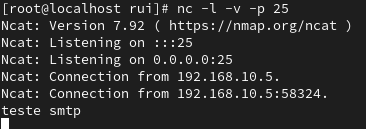
\includegraphics[scale=0.5]{btw/btw_smtp_dmz.png}
    \caption{Netcat command DMZ's smtp server}
    \label{fig:network-arc}
\end{figure}

\begin{figure}[H]
    \centering
    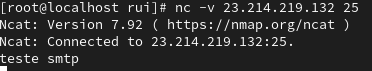
\includegraphics[scale=0.5]{btw/btw_smtp_internal.png}
    \caption{Netcat command internal network}
    \label{fig:network-arc}
\end{figure}

\subsubsection{POP and IMAP connections to the mail server.}
\quad 
To allow POP3 (Post Office Protocol 3) and IMAP (Internet Message Access Protocol)  we created the following rules:

\texttt{}\par
\texttt{iptables -A FORWARD -d 23.214.219.131 -p tcp --dport pop3 -j ACCEPT}\par
\texttt{iptables -A FORWARD -s 23.214.219.131 -p tcp --sport pop3 -j ACCEPT}\par
\texttt{}\par
\texttt{}\par
\texttt{iptables -A FORWARD -d 23.214.219.131 -p tcp --dport imap -j ACCEPT}\par
\texttt{iptables -A FORWARD -s 23.214.219.131 -p tcp --sport imap -j ACCEPT}\par
\texttt{}\par


To test we use the next netcat commands:
\texttt{}\par
\texttt{}\par
DMZ (mail server) POP3: \texttt{nc -l -v -p 110} \par
Internal Network POP3: \texttt{nc -v 23.214.219.131 110} \par
\texttt{}\par
\texttt{}\par
DMZ (mail server) IMAP: \texttt{nc -l -v -p 143} \par
Internal Network IMAP: \texttt{nc -v 23.214.219.131 143} \par
\texttt{}\par
\begin{figure}[H]
    \centering
    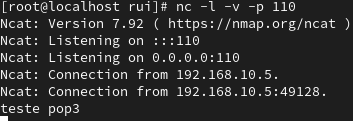
\includegraphics[scale=0.5]{btw/btw_pop3_dmz.png}
    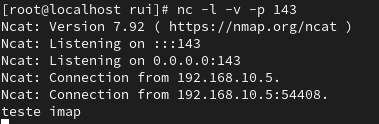
\includegraphics[scale=0.5]{btw/btw_imap_dmz.png}
    \caption{Netcat command DMZ's mail server}
    \label{fig:network-arc}
\end{figure}

\begin{figure}[H]
    \centering
    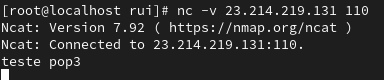
\includegraphics[scale=0.5]{btw/btw_pop3_internal.png}
    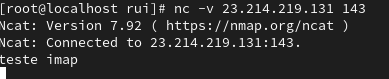
\includegraphics[scale=0.5]{btw/btw_imap_internal.png}
    \caption{Netcat command internal network}
    \label{fig:network-arc}
\end{figure}



\subsubsection{HTTP and HTTPS connections to the www server}

To allow POP3 (Post Office Protocol 3) and IMAP (Internet Message Access Protocol)  we created the following rules:

\texttt{}\par
\texttt{iptables -A FORWARD -d 23.214.219.133 -p tcp --dport http -j ACCEPT}\par
\texttt{iptables -A FORWARD -s 23.214.219.133 -p tcp --sport http -j ACCEPT}\par
\texttt{}\par
\texttt{}\par
\texttt{iptables -A FORWARD -d 23.214.219.133 -p tcp --dport https -j ACCEPT}\par
\texttt{iptables -A FORWARD -s 23.214.219.133 -p tcp --sport https -j ACCEPT}\par
\texttt{}\par


To test we use the next netcat commands:
\texttt{}\par
\texttt{}\par
DMZ (www server) HTTP: \texttt{nc -l -v -p 80} \par
Internal Network HTTP: \texttt{nc -v 23.214.219.133 80} \par
\texttt{}\par
\texttt{}\par
DMZ (www server) HTTPS: \texttt{nc -l -v -p 443} \par
Internal Network HTTPS: \texttt{nc -v 23.214.219.133 443} \par
\texttt{}\par
\begin{figure}[H]
    \centering
    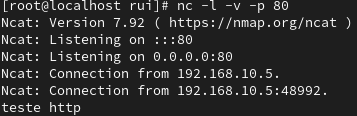
\includegraphics[scale=0.5]{btw/btw_http_dmz.png}
    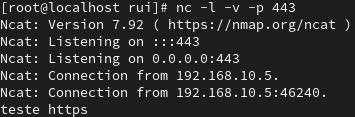
\includegraphics[scale=0.5]{btw/btw_https_dmz.png}
    \caption{Netcat command DMZ's www server}
    \label{fig:network-arc}
\end{figure}

\begin{figure}[H]
    \centering
    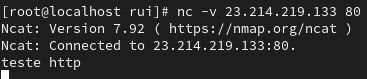
\includegraphics[scale=0.5]{btw/btw_http_internal.png}
    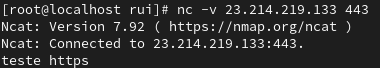
\includegraphics[scale=0.5]{btw/btw_https_internal.png}
    \caption{Netcat command internal network}
    \label{fig:network-arc}
\end{figure}


\subsubsection{OpenVPN connections to the vpn-gw server}

\quad To enable connections from the OpenVPN (open-source virtual private network) we created the following rules:

\texttt{}\par
\texttt{iptables -A FORWARD -d 23.214.219.134 -p tcp --dport openvpn -j ACCEPT}\par
\texttt{iptables -A FORWARD -s 23.214.219.134 -p tcp --sport openvpn -j ACCEPT}\par
\texttt{}\par


In order to test these we used the netcat command:
\texttt{}\par
\texttt{}\par
DMZ (vpn-gw server): \texttt{nc -l -v -p 1194} \par
Internal Network: \texttt{nc -v 23.214.219.134 1194} \par
\texttt{}\par
\begin{figure}[H]
    \centering
    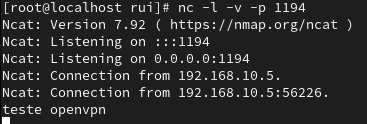
\includegraphics[scale=0.5]{btw/btw_openvpn_dmz.png}
    \caption{Netcat command DMZ's vpn-gw server}
    \label{fig:network-arc}
\end{figure}

\begin{figure}[H]
    \centering
    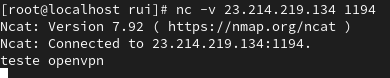
\includegraphics[scale=0.5]{btw/btw_openvpn_internal.png}
    \caption{Netcat command internal network}
    \label{fig:network-arc}
\end{figure}


\subsubsection{VPN clients connected to the gateway (vpn-gw) should be able to connect to all services in the Internal network (assume 
the gateway does SNAT/MASQUERADING for communications received from clients).}
\quad Here we want to allow all users connected to the vpn server to have access to the services in the internal network, so the next rules were created:


\texttt{}\par
\texttt{iptables -A FORWARD -s 23.214.219.134 -d 192.168.10.0/24 -p tcp -j ACCEPT }\par
\texttt{iptables -A FORWARD -d 23.214.219.134 -s 192.168.10.0/24 -p tcp -j ACCEPT}\par
\texttt{}\par


In order to test these we used the netcat command:
\texttt{}\par
\texttt{}\par
DMZ (vpn-gw server): \texttt{nc -v 192.168.10.6 1234} \par
Internal Network (datastore): \texttt{nc -l -v -p 1234} \par
\texttt{}\par
\begin{figure}[H]
    \centering
    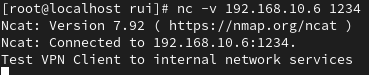
\includegraphics[scale=0.5]{btw/btw_vpn_client_dmz.png}
    \caption{Netcat command DMZ's vpn-gw server}
    \label{fig:network-arc}
\end{figure}

\begin{figure}[H]
    \centering
    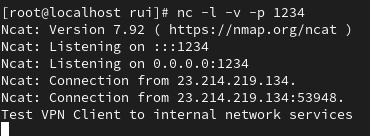
\includegraphics[scale=0.5]{btw/btw_vpn_client_internal.png}
    \caption{Netcat command internal network (datastore)}
    \label{fig:network-arc}
\end{figure}




\subsection{Firewall configuration for connections to the external IP address of the firewall (using NAT)}
\quad In this part of the assignment we want to authorize all connections originated in the outside and destined to the external IP address. So we are going to use DNAT.


\subsubsection{FTP connections (in passive and active modes) to the ftp server}
\quad Here we want to configure our firewall in order to allow FTP connections in passive and active modes. The case of FTP is different than what we've done for the other protocols, since with the other protocols we only worry about one port, and in this case we need to create rules to port 20 (ftp), 21 (ftp-data) and 60000:60099 (range of high ports that we defined in the ftp server configuration) and then use DNAT to redirect the ftp connections to the external IP address to the ftp server in the internal network. To do so, we use the following commands:

\texttt{}\par
\texttt{iptables -t nat -A PREROUTING -s 87.248.214.0/24 -d 87.248.214.97 -p tcp --dport ftp -j DNAT --to-destination 192.168.10.5}\par
\texttt{iptables -A FORWARD -d 192.168.10.5 -p tcp --dport ftp -j ACCEPT}\par
\texttt{iptables -A FORWARD -s 192.168.10.5 -p tcp --sport ftp -j ACCEPT}\par
\texttt{iptables -A FORWARD -d 192.168.10.5 -p tcp --dport ftp-data -j ACCEPT}\par
\texttt{iptables -A FORWARD -s 192.168.10.5 -p tcp --sport ftp-data -j ACCEPT}\par
\texttt{iptables -t nat -A PREROUTING -s 87.248.214.0/24 -d 87.248.214.97 -p tcp --dport 60000:60099 -m conntrack --ctstate RELATED,ESTABLISHED -j DNAT --to-destination 192.168.10.5
}\par
\texttt{iptables -A FORWARD -d 87.248.214.97 -p tcp --dport 60000:60099 -m conntrack --ctstate RELATED,ESTABLISHED -j ACCEPT
}\par
\texttt{iptables -A FORWARD -d 87.248.214.97 -p tcp --sport 60000:60099 -m conntrack --ctstate RELATED,ESTABLISHED -j ACCEPT
}\par
\texttt{}\par

In addicion to the rules, we need some commands which are:
\begin{itemize}
    \item \texttt{modprobe nf_conntrack_ftp}
    \item \texttt{modprobe nf_nat_ftp}
    \item \texttt{echo 1 > /proc/sys/net/netfilter/nf_conntrack_helper}
\end{itemize}

In order to test these we created an ftp server in the internal network using vsftp and connected to the router's external ip from a external ip address:
\texttt{}\par
\texttt{}\par
External Network: \texttt{ftp 87.248.214.97} \par
\texttt{}\par
\begin{figure}[H]
    \centering
    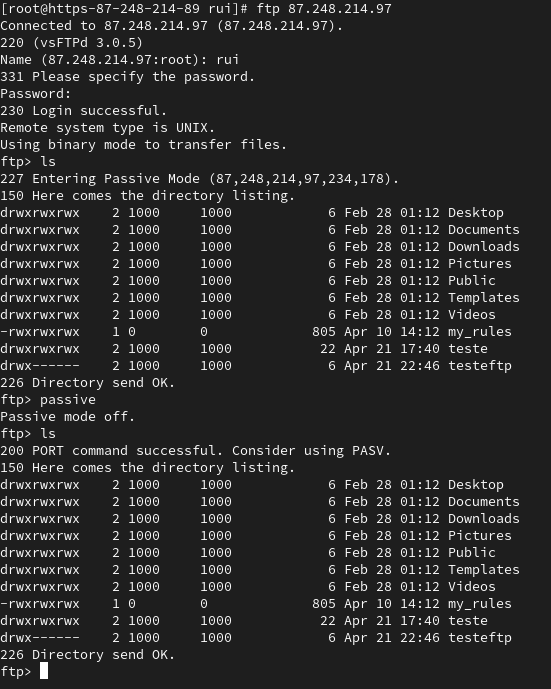
\includegraphics[scale=0.5]{out/out_ftp.png}
    \caption{Ftp connection from the external network in active and passive modes}
    \label{fig:network-arc}
\end{figure}

\subsubsection{SSH connections to the datastore server, but only if originated at the eden or dns2 servers}
\quad Here, we want to create rules that allow connections from the eden and dns2 servers to the datastore server in the internal network using DNAT.

\texttt{}\par
\texttt{iptables -t nat -A PREROUTING -s 193.136.212.1 -d 87.248.214.97 -p tcp --dport ssh -j DNAT --to-destination 192.168.10.6}\par
\texttt{iptables -A FORWARD -s 193.136.212.1 -d 192.168.10.6 -p tcp --dport ssh -j ACCEPT}\par
\texttt{iptables -A FORWARD -s 192.168.10.6 -d 193.136.212.1 -p tcp --sport ssh -j ACCEPT}\par
\texttt{iptables -t nat -A PREROUTING -s 193.137.16.75 -d 87.248.214.97 -p tcp --dport ssh -j DNAT --to-destination 192.168.10.6}\par
\texttt{iptables -A FORWARD -s 193.137.16.75 -d 192.168.10.6 -p tcp --dport ssh -j ACCEPT}\par
\texttt{iptables -A FORWARD -s 192.168.10.6 -d 193.137.16.75 -p tcp --sport ssh -j ACCEPT}\par
\texttt{}\par

In order to test these, we created new rules to simulate eden and dns2 servers (the rules are all the same, the only thing changing is the ip address of the source of the connection):

\texttt{iptables -t nat -A PREROUTING -s 87.248.214.89 -d 87.248.214.97 -p tcp --dport ssh -j DNAT --to-destination 192.168.10.6}\par
\texttt{iptables -A FORWARD -s 87.248.214.89 -d 192.168.10.6 -p tcp --dport ssh -j ACCEPT}\par
\texttt{iptables -A FORWARD -s 192.168.10.6 -d 87.248.214.89 -p tcp --sport ssh -j ACCEPT}\par
\texttt{}\par



\texttt{}\par
\texttt{}\par
External Network: \texttt{ssh rui@87.248.214.97} \par
\texttt{}\par
\begin{figure}[H]
    \centering
    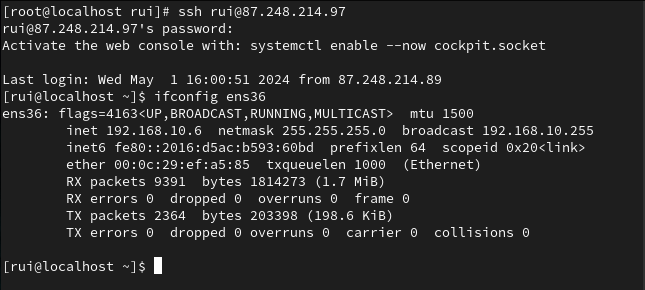
\includegraphics[scale=0.5]{out/out_ssh_from_dns_servers.png}
    \caption{ssh from the external network}
    \label{fig:network-arc}
\end{figure}


\subsection{Firewall configuration for communications from the internal network to the outside (using NAT)}
\quad In this part of the assignment we want to authorize all connections originated in the internal network and destined to the outside. So we are going to use SNAT.
\subsubsection{Domain name resolutions using DNS}
\quad Here we want to allow dns requests from the internal network to the Internet, using SNAT.


\texttt{}\par
\texttt{iptables -A FORWARD -p udp -s 192.168.10.0/24 -d 87.248.214.0/24 --dport domain -j ACCEPT}\par
\texttt{iptables -A FORWARD -p udp -d 192.168.10.0/24 -s 87.248.214.0/24 --sport domain -j ACCEPT}\par
\texttt{iptables -t nat -A POSTROUTING -p udp -s 192.168.10.0/24 -d 87.248.214.0/24 --dport domain -j SNAT --to-source 87.248.214.97}\par
\texttt{iptables -A FORWARD -p tcp -s 192.168.10.0/24 -d 87.248.214.0/24 --dport domain -j ACCEPT}\par
\texttt{iptables -A FORWARD -p tcp -d 192.168.10.0/24 -s 87.248.214.0/24 --sport domain -j ACCEPT}\par
\texttt{iptables -t nat -A POSTROUTING -p tcp -s 192.168.10.0/24 -d 87.248.214.0/24 --dport domain -j SNAT --to-source 87.248.214.97}\par
\texttt{}\par


To test we use the next netcat commands:
\texttt{}\par
\texttt{}\par
External network UDP: \texttt{nc -l -v -u -p 53} \par
Internal Network UDP: \texttt{nc -v -u 87.248.214.89 53} \par
\texttt{}\par
\texttt{}\par
External network TCP: \texttt{nc -l -v -p 53} \par
Internal Network TCP: \texttt{nc -v 87.248.214.89 53} \par
\texttt{}\par
\begin{figure}[H]
    \centering
    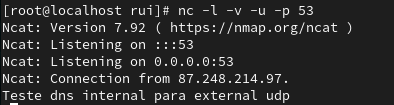
\includegraphics[scale=0.5]{out/out_dns_external_udp.png}
    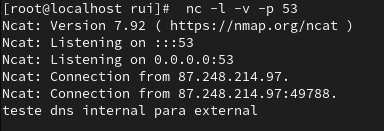
\includegraphics[scale=0.5]{out/out_dns_external.png}
    \caption{Netcat command External network}
    \label{fig:network-arc}
\end{figure}

\begin{figure}[H]
    \centering
    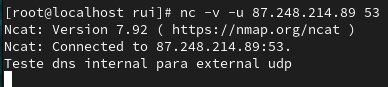
\includegraphics[scale=0.5]{out/out_dns_internal_udp.png}
    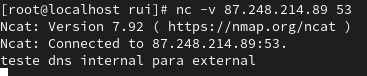
\includegraphics[scale=0.5]{out/out_dns_internal.png}
    \caption{Netcat command internal network}
    \label{fig:network-arc}
\end{figure}



\subsubsection{HTTP, HTTPS and SSH connections}
\quad Now we need to create rules to allow http, https and ssh traffic that comes from the internal network to Internet using SNAT.

\texttt{}\par
\texttt{iptables -t nat -A POSTROUTING -p tcp -s 192.168.10.0/24 -d 192.168.93.0/24 --dport http -j SNAT --to-source 192.168.93.128 }\par
\texttt{iptables -A FORWARD -p tcp -s 192.168.10.0/24 -d 87.248.214.0/24   --dport http -j ACCEPT}\par
\texttt{iptables -A FORWARD -p tcp -d 192.168.10.0/24 -s 87.248.214.0/24   --sport http -j ACCEPT}\par
\texttt{}\par
\texttt{}\par
\texttt{iptables -t nat -A POSTROUTING -p tcp -s 192.168.10.0/24 -d  87.248.214.0/24 --dport https -j SNAT --to-source 87.248.214.97}\par
\texttt{iptables -A FORWARD -p tcp -s 192.168.10.0/24 -d 87.248.214.0/24   --dport https -j ACCEPT}\par
\texttt{iptables -A FORWARD -p tcp -d 192.168.10.0/24 -s 87.248.214.0/24   --sport https -j ACCEPT}\par
\texttt{}\par
\texttt{}\par
\texttt{iptables -t nat -A POSTROUTING -p tcp -s 192.168.10.0/24 -d  87.248.214.0/24 --dport ssh -j SNAT --to-source 87.248.214.97}\par
\texttt{iptables -A FORWARD -p tcp -s 192.168.10.0/24 -d 87.248.214.0/24   --dport ssh -j ACCEPT}\par
\texttt{iptables -A FORWARD -p tcp -d 192.168.10.0/24 -s 87.248.214.0/24   --sport ssh -j ACCEPT}\par
\texttt{}\par

To test we used the nectat command for http and https and ssh command for ssh:
\texttt{}\par
\texttt{}\par
External network http: \texttt{nc -l -v -p 80} \par
Internal Network http: \texttt{nc -v 87.248.214.89 80} \par
\texttt{}\par
\texttt{}\par
External network https: \texttt{nc -l -v -p 443} \par
Internal Network https: \texttt{nc -v 87.248.214.89 443} \par
\texttt{}\par
\begin{figure}[H]
    \centering
    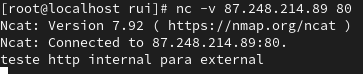
\includegraphics[scale=0.5]{out/out_http_snat_internal.png}
    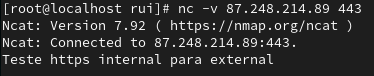
\includegraphics[scale=0.5]{out/out_https_snat_internal.png}
    \caption{Netcat command internal network}
    \label{fig:network-arc}
\end{figure}

\begin{figure}[H]
    \centering
    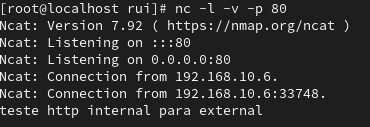
\includegraphics[scale=0.5]{out/out_http_snat_external.png}
    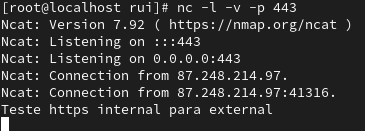
\includegraphics[scale=0.5]{out/out_https_snat_external.png}
    \caption{Netcat command external network}
    \label{fig:network-arc}
\end{figure}
\texttt{}\par

\texttt{}\par
Internal Network SSH: \texttt{ssh rui@87.248.214.89} \par
\texttt{}\par
\begin{figure}[H]
    \centering
    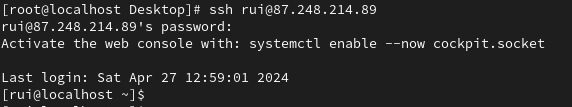
\includegraphics[scale=0.5]{out/out_ssh_internal_to_external_sshcommand.png}
    \caption{ssh command internal network}
    \label{fig:network-arc}
\end{figure}

\subsubsection{FTP connections (in passive and active modes) to external FTP servers}
\quad In this topic we want to allow ftp connections from the internal network to an external network ftp server.

\texttt{}\par
\texttt{iptables -t nat -A POSTROUTING -s 192.168.10.0/24 -d 87.248.214.0/24 -p tcp --dport ftp -j SNAT --to-source 87.248.214.97}\par
\texttt{iptables -A FORWARD -d 87.248.214.0/24 -p tcp --dport ftp -j ACCEPT}\par
\texttt{iptables -A FORWARD -s 87.248.214.0/24 -p tcp --sport ftp -j ACCEPT}\par
\texttt{iptables -A FORWARD -s 87.248.214.0/24 -p tcp --sport ftp-data -j ACCEPT}\par
\texttt{iptables -A FORWARD -d 87.248.214.0/24 -p tcp --dport ftp-data -j ACCEPT}\par
\texttt{iptables -t nat -A POSTROUTING -s 192.168.10.0/24 -d 87.248.214.0/24 -p tcp --dport 60000:60099 -m conntrack --ctstate RELATED,ESTABLISHED -j SNAT --to-source 87.248.214.97}\par
\texttt{iptables -A FORWARD -d 87.248.214.0/24 -p tcp --dport 60000:60099 -m conntrack --ctstate RELATED,ESTABLISHED -j ACCEPT}\par
\texttt{iptables -A FORWARD -d 87.248.214.0/24 -p tcp --sport 60000:60099 -m conntrack --ctstate RELATED,ESTABLISHED -j ACCEPT}\par
\texttt{iptables -A FORWARD -d 192.168.10.0/24 -p tcp --dport 60000:60099 -m conntrack --ctstate RELATED,ESTABLISHED -j ACCEPT}\par
\textttiptables -A FORWARD -d 192.168.10.0/24 -p tcp --sport 60000:60099 -m conntrack --ctstate RELATED,ESTABLISHED -j ACCEPT{}\par
\texttt{}\par

In order to test these we created an ftp server in the external network using vsftp and connected from the internal network:\par
\texttt{}\par
Internal Network: \texttt{ftp 87.248.214.89} \par
\texttt{}\par
\begin{figure}[H]
    \centering
    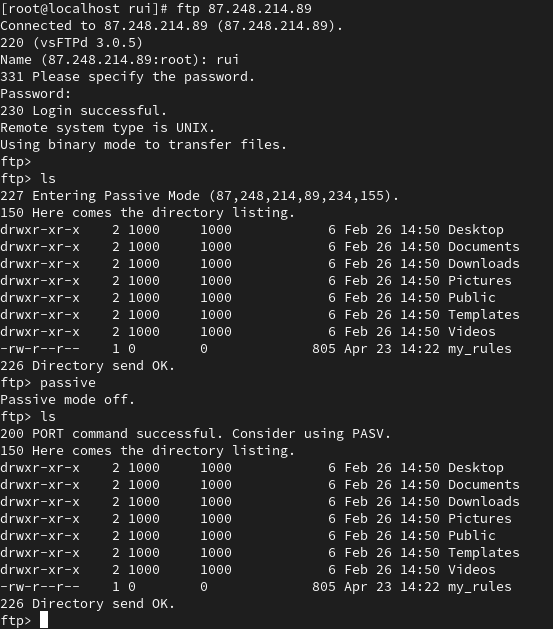
\includegraphics[scale=0.5]{out/out_ftp_snat.png}
    \caption{ftp command internal network}
    \label{fig:network-arc}
\end{figure}




\section{Suricata}
\quad The last requirement of this assignment is to enable in the firewall system, the capability to detect and react to security attacks. To be more specific, we want to be able to detect and react to the following attacks:
\begin{itemize}
    \item Two types of SQL injection.
    \item Two types of DoS (Denial of Service) attacks.
    \item OS fingerprinting attempts.
\end{itemize}

\subsection{Suricata configuration}
\quad TO configure suricata we need to add our rules to a file and specify in the suricata.yaml file where the rules are. In addiction to that, in the same yaml file we need to change the capture settings in the \texttt{af_packet} section, and the network information in \texttt{HOME_NET}.



\texttt{}\par
\begin{figure}[H]
    \centering
    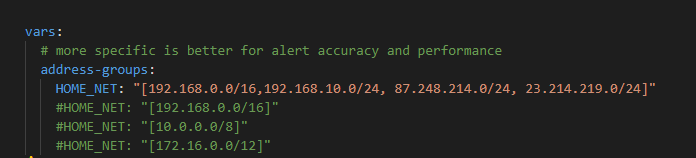
\includegraphics[scale=0.5]{suricata/config_home_net.png}
    \caption{HOME_NET}
    \label{fig:network-arc}
\end{figure}

\texttt{}\par
\begin{figure}[H]
    \centering
    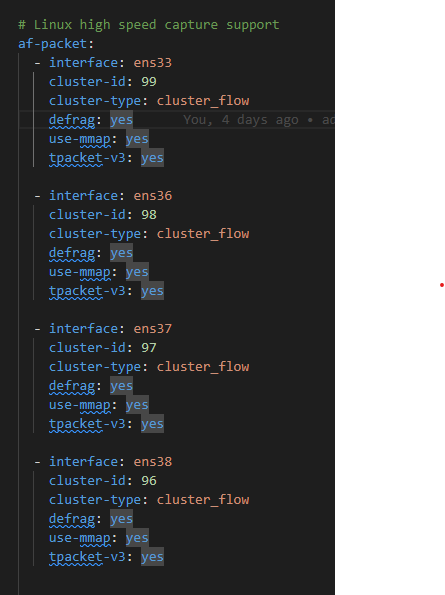
\includegraphics[scale=0.5]{suricata/config_af_packet.png}
    \caption{af-packet}
    \label{fig:network-arc}
\end{figure}


\texttt{}\par
\begin{figure}[H]
    \centering
    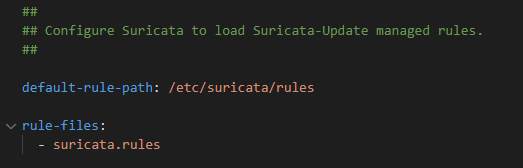
\includegraphics[scale=0.5]{suricata/config_path.png}
    \caption{suricata.rules path}
    \label{fig:network-arc}
\end{figure}

After this we need to add one rule to IPTables in order to have all the traffic go throw a queue and be analyzed in Suricata.
\texttt{}\par
\texttt{iptables -I FORWARD -j NFQUEUE --queue-num 0}\par
\texttt{}\par
And now we add the rules to the suricata.rules file:
\begin{itemize}
    \item SQL injection:\par
    \texttt{drop tcp any any -> any any (msg:"SQL Injection type drop table detected"; content:"drop table"; sid:1; rev:1;)}\par
    \texttt{drop tcp any any -> any any (msg: "SQL Injection type 1=1 detected"; pcre: "/OR+( )+[0-9]+( )*+=+( )*+[0-9]+/"; sid:2;)}\par
    \texttt{}\par
    The first rule is to detect and drop a message containing a "drop table" query. The second one detects if a query has the "OR 1=1" using a regular expression. \par
    

    \item DOS atacks:\par
    \texttt{alert udp any any -> 192.168.10.0/24 any (msg:"ALERT UDP Flood"; threshold:type both, track by_dst, count 15, seconds 3; sid:1000001; rev:1;)}\par
    \texttt{alert tcp any any -> 192.168.10.0/24 any (msg:"ALERT TCP Flood"; threshold:type both, track by_dst, count 15, seconds 3; sid:1000005; rev:1;)}\par

    \texttt{}\par
    Here we are detecting both TCP and UDP flooding attacks.\par


    \item OS Fingerprint:\par
    \texttt{alert tcp any any -> any any (msg:"OS Fingerprinting Detected: NMAP"; flags:FPU;reference:}\par
    \texttt{url,nmap.org; sid:6; rev:1;)}\par

    \texttt{}\par
    This rule is to detect OS fingerprinting attacks via NMAP with the flag -sX.  
    
    \texttt{}\par
\end{itemize}

All the rules follow the sintaxe mentioned in \ref{subsec:suricata}. We used \textbf{alert} and \textbf{drop actions} that are generate an alert when the conditions are met and drop the packet and generate an alert respectively.\par
We used both \textbf{TCP} and \textbf{UDP} protocols, however each rule uses or tcp or udp, so if the rule uses \textbf{tcp} and the attack is performed using \textbf{udp} it will not be detected. \par
The source ip and source ports were always \textbf{any} which means that the rules apply to all incoming IP's and ports. About the destination ports and IP's we also used \textbf{any} except in the DOS attacks where we specify a range of IP's.\par
Then we have the \textbf{msg} that is what appears when Suricata detects that type of attack, the \textbf{sid} that is the rule ID, \textbf{rev} that is the revision number, the \textbf{pcre} which means Perl Compatible Regular Expressions that is used to identify regular expressions, in our case the expression \texttt{ "/OR+( )+[0-9]+( )*+=+( )*+[0-9]+/"} is used to identify \textbf{OR 1=1}, the \textbf{content} which have a string to verify if it is in the message's content. The other parameters like \textbf{flags} and \textbf{threshold} are more specific to some types of rules.


\subsection{Tests}

In order to test those rules we need to start suricata and connect it to the queue (NFQUEUE) using the command:\par
\texttt{sudo suricata -c /etc/suricata/suricata.yaml -q 0}\par
\texttt{}\par

To test SQL Injection we used netcat:\par
\begin{itemize}
    \item Drop Table attack\par

\texttt{}\par
\begin{figure}[H]
    \centering
    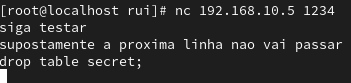
\includegraphics[scale=0.5]{suricata/sur_sqli_drop_table_external.png}
    \caption{Drop Table query being in the sender}
    \label{fig:network-arc}
\end{figure}


\texttt{}\par
\begin{figure}[H]
    \centering
    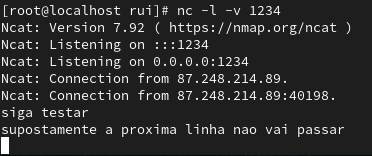
\includegraphics[scale=0.5]{suricata/sur_sqli_drop_table_internal.png}
    \caption{Drop Table in the receiver}
    \label{fig:network-arc}
\end{figure}


\texttt{}\par
\begin{figure}[H]
    \centering
    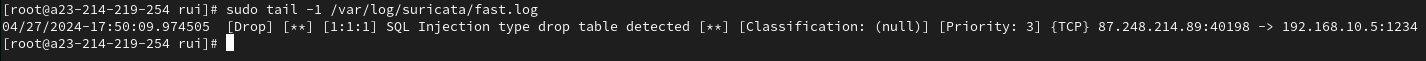
\includegraphics[scale=0.45]{suricata/sur_sqli_drop_table_log.png}
    \caption{Log - /var/log/suricata/fast.log}
    \label{fig:network-arc}
\end{figure}


\item 1=1 atack\par

\texttt{}\par
\begin{figure}[H]
    \centering
    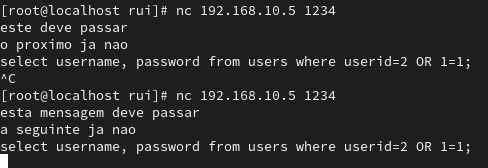
\includegraphics[scale=0.5]{suricata/sur_sqli_1eq1_external.png}
    \caption{Drop Table query being in the sender}
    \label{fig:network-arc}
\end{figure}


\texttt{}\par
\begin{figure}[H]
    \centering
    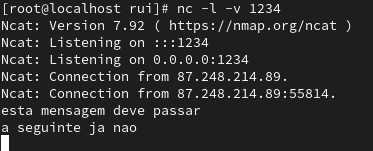
\includegraphics[scale=0.5]{suricata/sur_sqli_1eq1_internal.png}
    \caption{Drop Table in the receiver}
    \label{fig:network-arc}
\end{figure}


\texttt{}\par
\begin{figure}[H]
    \centering
    \includegraphics[scale=0.45]{suricata/sur_sqli_1eq1_log.png}
    \caption{Log - /var/log/suricata/fast.log}
    \label{fig:network-arc}
\end{figure}
\end{itemize}


To test DOS attacks we used hping3 command:

\begin{itemize}
    \item UDP flood:\par
    \texttt{hping3 -S -p 80 -2 --flood 192.168.10.6}

    \texttt{}\par

\texttt{}\par
\begin{figure}[H]
    \centering
    \includegraphics[scale=0.5]{suricata/sur_DoS_udp_external.png}
    \caption{Drop Table in the sender}
    \label{fig:network-arc}
\end{figure}


\texttt{}\par
\begin{figure}[H]
    \centering
    \includegraphics[scale=0.45]{suricata/sur_DoS_udp_log.png}
    \caption{Log - /var/log/suricata/fast.log}
    \label{fig:network-arc}
\end{figure}


\item TCP flood:\par
\texttt{hping3 -S -p 80 --flood 192.168.10.6}
\texttt{}\par
\begin{figure}[H]
    \centering
    \includegraphics[scale=0.5]{suricata/sur_DoS_tcp_external.png}
    \caption{Drop Table in the sender}
    \label{fig:network-arc}
\end{figure}


\texttt{}\par
\begin{figure}[H]
    \centering
    \includegraphics[scale=0.45]{suricata/sur_DoS_tcp_log.png}
    \caption{Log - /var/log/suricata/fast.log}
    \label{fig:network-arc}
\end{figure}

\end{itemize}


To test OS fingerprint attacks we use nmap:\par

\texttt{nmap -sX --system-dns -p 80 192.168.10.6}
\texttt{}\par
\begin{figure}[H]
    \centering
    \includegraphics[scale=0.5]{suricata/os_fingertip_nmap_external.png}
    \caption{nmap command in the sender}
    \label{fig:network-arc}
\end{figure}


\texttt{}\par
\begin{figure}[H]
    \centering
    \includegraphics[scale=0.45]{suricata/os_fingertip_nmap_log.png}
    \caption{Log - /var/log/suricata/fast.log}
    \label{fig:network-arc}
\end{figure}



\section{Conclusion}
\quad To conclude, this assignment has successfully demonstrated the practical application of IPTables and Suricata in creating a secure network environment. With it we learn how to create IPTables rules and create rules to detect sql injection, dos and os fingerprint attacks. To validate our configuration we did a set of tests and with that we believe that the assignment requirements were sucessfully implemented.





\begin{thebibliography}{}
\bibitem{Slides}Information Tecnology Security Slides
\bibitem{livro_stor}Jorge Granjal, Segurança Prática em Sistemas e Redes com Linux, FCA, 2017

\bibitem{nethack}
Setup an OpenVPN server with certificate and two-factor authentication on CentOS 7 Retrieved March 8, 2023, from https://nethack.ch/2016/12/08/setup-an-openvpn-server-with-certificate-and-two-factor-authen\par tication-on-centos-7/

\bibitem{digitalocean} 
How the iptables firewall works, Retrieved April 22, 2024 from https://www.digitalocean.com/community/tutorials/how-the-iptables-firewall-works

\bibitem{suricata} Suricata Rules Format Retrieved April 27, 2024 from 
https://docs.suricata.io/en/suricata-6.0.3/rules/intro.html

\bibitem{winaero} Fix FTP access from Linux client PC with firewall enabled Retrieved April 25 from https://winaero.com/fix-ftp-access-from-linux-client-pc-with-firewall-enabled/

\bibitem{alibabacloud} iptables settings in vsftpd active /standby mode for Linux instances Retrieved April 25 from https://www.alibabacloud.com/help/en/ecs/iptables-settings-in-vsftpd-active-or-standby-mode-for-linux-instances
\bibitem{NMAP} TCP FIN, NULL, and Xmas Scans Retrieved April 29, 2024 from
https://nmap.org/book/scan-methods-null-fin-xmas-scan.html
\bibitem{linuxmint} DOS Flood With hping3 Retrieved April 29, 2024 from
https://linuxhint.com/hping3/


\bibitem{medium} DDoS Attack Detection with Suricata Retrieved April 29 from https://medium.com/@mshulkhan/detection-attack-using-suricata-1-5ea7b2f62551

\bibitem{w3schools} Sql Injection Retrieved April 29 from  https://www.w3schools.com/sql/sql\_injection.asp


\end{thebibliography}

\end{document}